\documentclass[12pt,a4paper]{article}
\usepackage[utf8]{inputenc}
\usepackage[swedish]{babel}
\usepackage{amsmath}
\usepackage{amsfonts}
\usepackage{amssymb}
\usepackage[affil-it]{authblk}
\usepackage{subcaption}
\usepackage[innercaption]{sidecap}
%\usepackage{floatrow}
\usepackage{float}
\usepackage{movie15}

\RequirePackage{color,graphicx}
\usepackage{hyperref}
\usepackage{cleveref}

\definecolor{linkcolor}{rgb}{0,0.2,0.6}
\hypersetup{colorlinks,breaklinks,urlcolor=linkcolor,linkcolor = linkcolor} 
\usepackage{blindtext}
\graphicspath{{C:/Users/danne/Pictures/}}

\begin{document}

\author{Rasmus Svensson%
  \thanks{E-mail: \href{mailto:rasmus.sjobol@gmail.com}{rasmus.sjobol@gmail.com}}, \ {Daniel Holmkvist%
  \thanks{E-mail: \href{mailto:dh222kd@student.lnu.se}{dh222kd@student.lnu.se}}}}
\title{Inlämningsuppgift 1 - 1DV005}
\maketitle
\tableofcontents
\newpage
\section{Scratchuppgifter}
\subsection{Uppgift 1: Euklides algoritm} 
Vår implementation börjar med att fråga användaren om två tal a,b (här används  Då vill vill att $ a \geq b$ byter vi värde på dem ifall detta ej uppfylls. Sedan använder vi (pseudokod): \\
WHILE b != 0         \\
 	rest = a mod b \\
	a = b \\
	b = rest \\ \\
Först används modulus för att beräkna resten, sedan genomförs Euklides algoritm tills resten från divisionen mellan a och b är 0. Euklides algoritm säger att när resten är 0 är svaret funnet och är a, så där slutas loopen, och svaret skrivs ut. \\

%\noindent\begin{minipage}{0.3\textwidth}% adapt widths of minipages to your needs
\begin{figure}[H]
	\label{fig:euk}
	\caption{Hela implementationen av Euklides algoritm}
	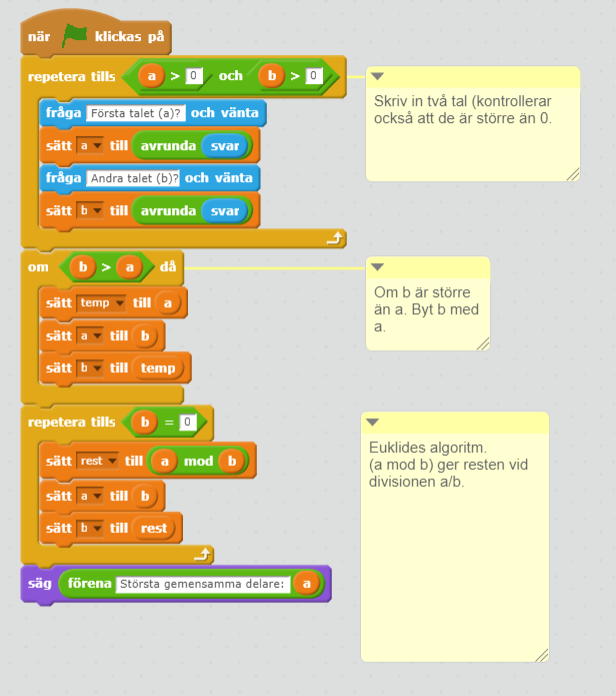
\includegraphics[scale=0.7]{euklidesimpl}
\end{figure}
%\end{minipage}%
%\hfill%

Länk till projektet:  \\
 \url{https://scratch.mit.edu/projects/178445830/#editor }
\subsection{Uppgift 2: Binärsökning}
På denna uppgiften har vi en sorterad lista på 10 olika heltal.
Vi implementerade algoritmen rekursivt. Binärsökning jämför det mellersta elementet i en lista med det som eftersöks (här kallat nyckeln). Då finns tre fall:    \\ \\
Fall 1. Värdet på mittenelementet i listan = nyckeln. Detta medför att elementet som söks har funnits, och vi kan skriva ut dess index.  \\
Fall 2. Värdet på mittenelementet $<$ nyckeln. Eftersom listan är sorterad måste elementets som söks ha ett större indexvärde än det vi nu kollar på, således räcker det att söka igenom den halvan av listan. Mittenelementet kan också uteslutas då det redan är känt från 1) att det inte är det värdet vi söker. \\
Fall 3. Värdet på mittenelementet $>$ nyckeln. Med samma resonemang som i fall 2 kan vi söka igenom endast den halvan som har ett mindre index än mittenelementet.\\ \\
Om värdet som söks ej hittades kan samma metod kallas igen, fast med nya gränser för de index som söks. De möjliga index en nyckel kan ha halveras således varje genomkörning. Indexet på det mellersta elementet inom gränserna max,min (heltal), fås genom  $(max + min)/2$. Detta värdet kan emellertid vara ett decimaltal, således avrundas det (här: alltid neråt, då det gör det enklare att följa koden). Scratchimplementationen för binärsökning finns att se som figur~\ref{fig2:binsearch}.

Om värdet inte finns med i listan kommer, vid något steg av genomsökningen värdet ligga utanför gränserna som söks, och då kan vi avbryta sökningen. 
\begin{figure}[H]
	\caption{Implementation av binärsökning}
	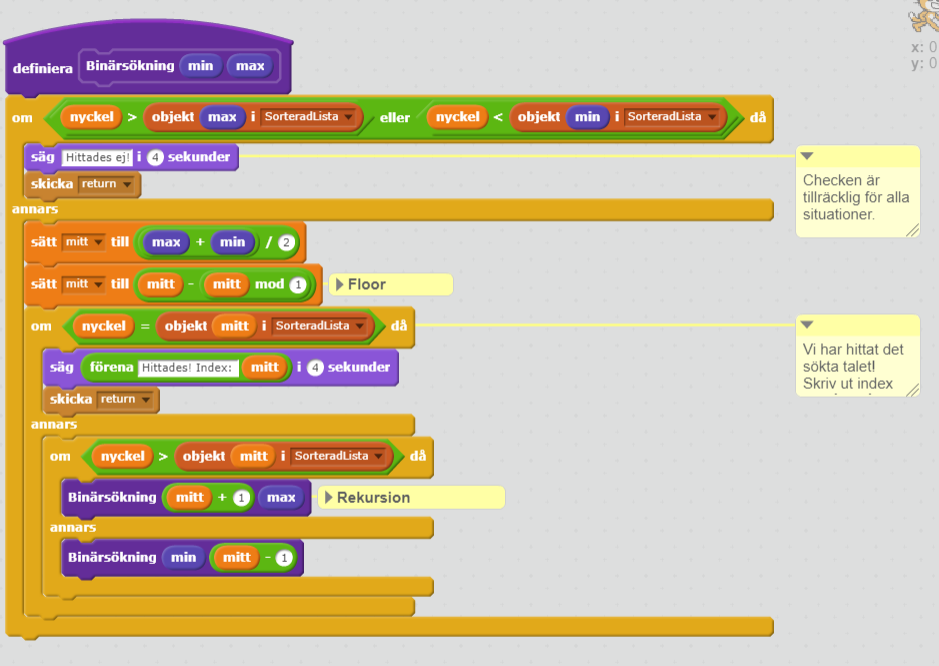
\includegraphics[scale=0.65]{binaryimpl}
	\label{fig2:binsearch}
\end{figure}
Länk till projektet: \\ \url{ https://scratch.mit.edu/projects/178458263/#editor } 
\subsection{Uppgift 3,4: Slumptal \& Urvalssortering}
För att lägga in slumpmässigt valda tal i listan används: \\
\begin{figure}[H]
	\caption{Lista av slumpmässiga tal}
	\centering
	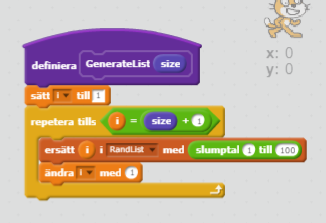
\includegraphics[scale=0.8]{listgen}
	\label{fig3:randlist} 
\end{figure}
I figur~\ref{fig3:randlist} läggs ett tal mellan 1-100 på första platsen, sedan andra, tills vi nått slutpunkten. Detta görs här genom en scratch-implementation av en for-loop, och användandet av scratch:s ``ersätt'' block.
 \\
Urvalssortering (eng: selection sort) hittar först det minsta talet, och sätter det först i listan, sedan det näst minsta, etc. Därför används två loopar, en för vilken position vi letar efter och en för att finna det minsta talet relevant för positionen. Om det finns ett relevant tal mindre än talet som står på platsen byts dessa genom en swap metod vilken byter plats på talen(se: figur~\ref{fig5:swap}).  \\
\begin{figure}[H]
	\caption{Urvalsortering}
	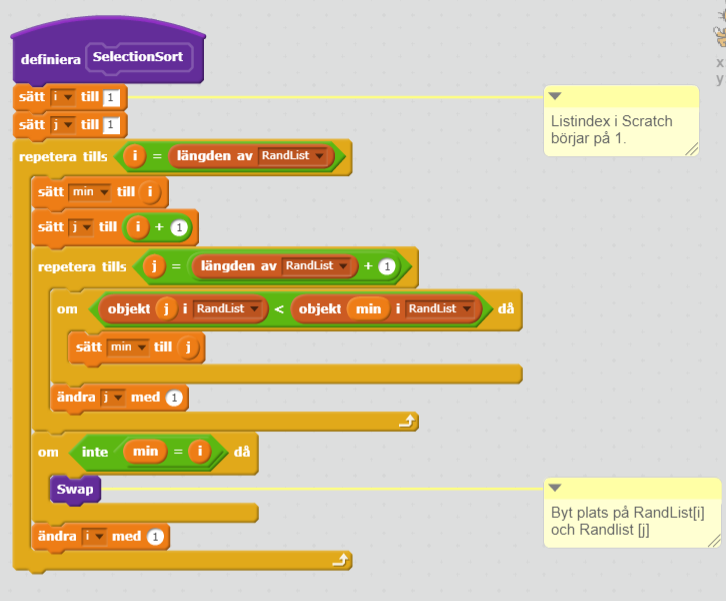
\includegraphics[scale=0.8]{selection}
	\label{fig4:selectionsort}
\end{figure}
\begin{figure}[H]
	\caption{Swap}
	\centering
	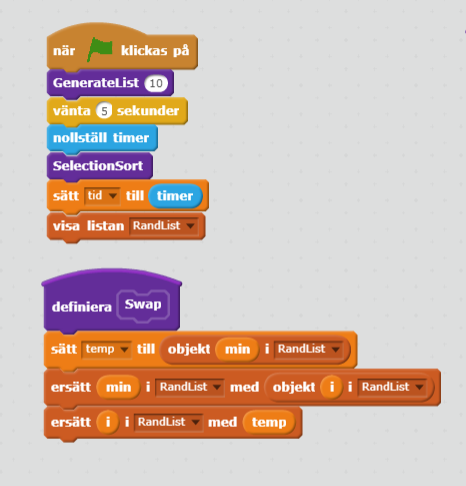
\includegraphics[scale=0.8]{swap}
	\label{fig5:swap}
\end{figure}
Länk till projektet:  \\
 \url{https://scratch.mit.edu/projects/178469197/#editor }
\subsection{Uppgift 5: Fibonaccis talföljd}
Då fibonaccitalen bygger på varandra kan vi, i enighet med dynamisk programmering, använda att vi vet Fib(n-1) och Fib(n-2) vid beräkning av Fib(n). På grund av att vi utgår ifrån talen 0,1 kommer detta alltid att vara tillräckligt. Vi kan således lägga ihop dessa och lägga in dem på rätt plats i listan. Man skulle kunna beräkna varje tal för sig självt, utan att ta hjälp av de tidigare beräkningarna, men det skulle vara en mycket ineffektiv lösning. Istället, genom användandet av dynamisk programmering har vi en betydligt bättre lösning, som bara kräver en addition för att få ut nästa tal.
\begin{figure}[H]
	\caption{Fibonaccitalen}
	\centering
	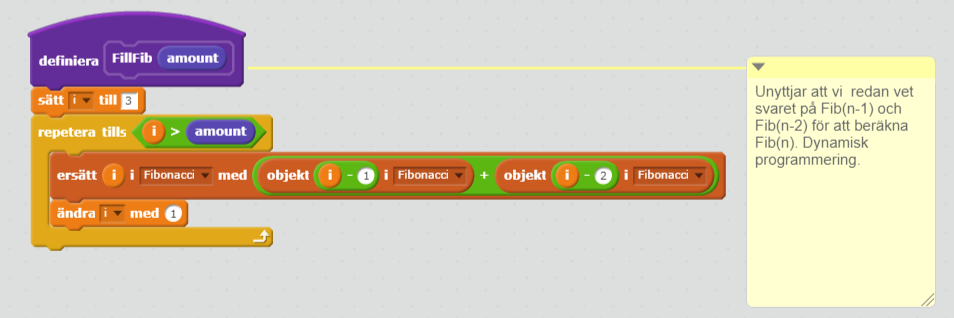
\includegraphics[scale=0.8]{fib}
	\label{fig6:fib}
\end{figure}
Länk till projektet:  \\
 \url{https://scratch.mit.edu/projects/178477056/#editor }
\section{Lego Mindstorms}
För uppgiften i lego mindstorms fanns flera delproblem som vi löste separat för att sedan foga samman dem till en användbar lösning till helhetsproblemet. \\
1. Följ linjen \\
2. Detektera kollision med hjulstapeln. \\
3. Plocka upp hjulen och vänd. \\
4. Följ linjen tillbaka och släpp hjulen \\
\subsection{Följa linjen}
Det största problemet av dessa var att få roboten att följa linjen. Först landade vi i en ganska enkel lösning, som svänger åt ena hållet om roboten är på linjen, annars åt det andra hållet (se: figur~\ref{fig7:switchfollow}). Detta fungerade emellertid, men resulterade i att roboten svängde konstant. Efter att övriga deluppgifter var lösta funderade vi över en möjlig lösning som istället kunde köra rakt när den var på linjen, men fortfarande följde den. Vi upptäckte att vi fick ett värde på ca. 50 när den stog på kanten, och att vi kunde använda det för att få den att köra rakt, på kanten, istället för på mitten av tejpen. 
\begin{figure}[H]
	\caption{Switch-följaren}
	\centering
	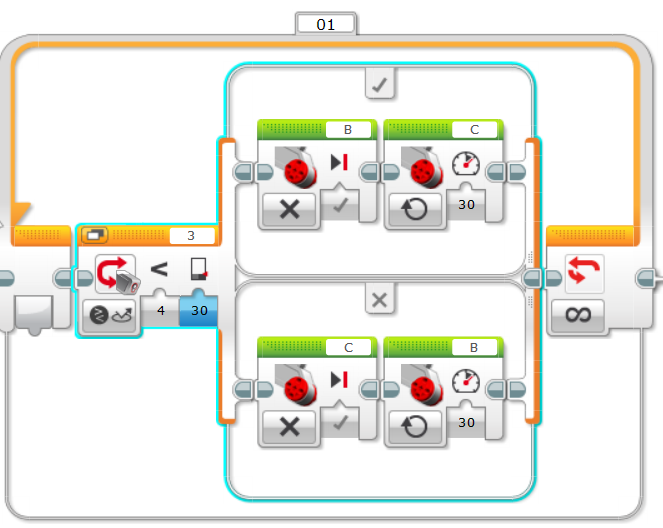
\includegraphics[scale=0.8]{switchfollow}
	\label{fig7:switchfollow}
\end{figure} 
\begin{figure}[H]
	\caption{Justerande}
	\centering
	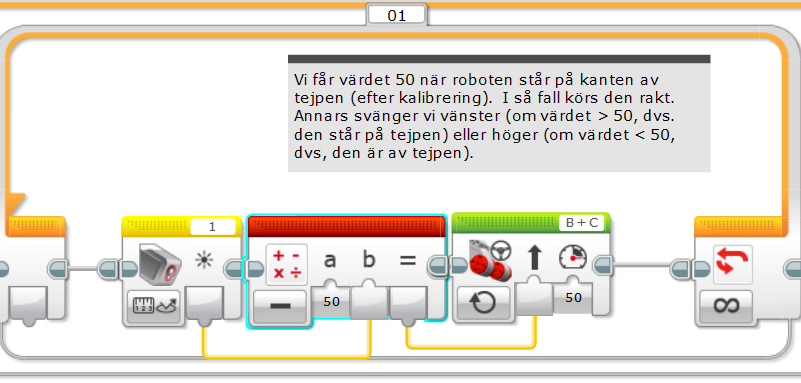
\includegraphics[scale=0.8]{legmindfollow}
	\label{fig8:linefollow}
\end{figure}
Hela lego mindstorms projektet finns som bilaga. 
\subsubsection{Kalibrering}
För att lösningen skulle fungera väl krävdes någon form av kalibrering, så att vi får ett användbart värde när den står på kanten. Därför 
\subsection{Detektion av hjulstapeln}

\section{Tidrapport}
9/10 -2017 1h /person. 
10/10 - 2017 1h / person. 
\end{document}
